\section{Introduction}
\label{sec:introduction}

% state the learning objective 
The objective of this laboratory assignment is to study a circuit containing 2 independent sources, $V_a$ and $I_d$, 1 voltage controlled source, $I_b$, 1 current controlled source, $V_c$, all of which are connected to 7 resistors. The circuit can be seen in Figure~\ref{fig1}.

\begin{figure}[h] \centering
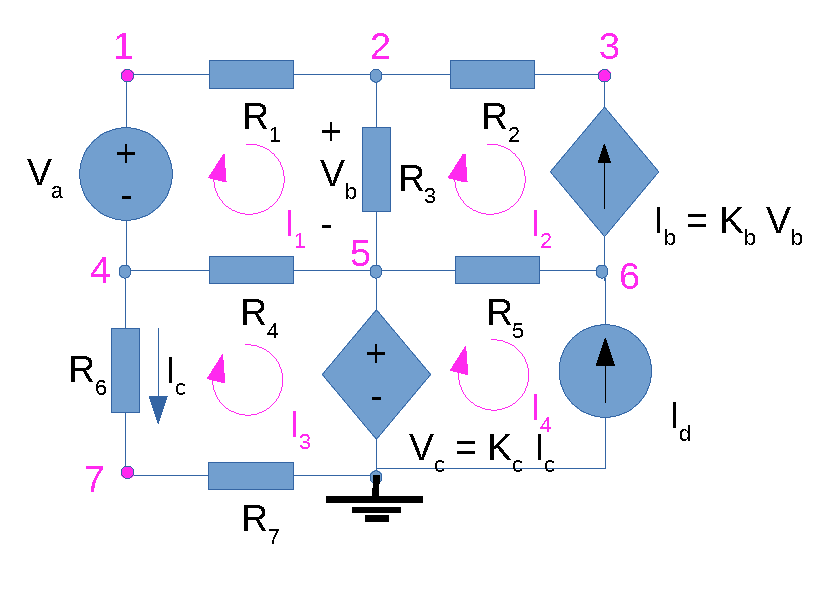
\includegraphics[width=0.4\linewidth]{t1-1.pdf}
\caption{A circuit containing many sources and resistors}
\label{fig1}
\end{figure}

In Section~\ref{sec:analysis}, a theoretical analysis of the circuit is
presented. In Section~\ref{sec:simulation}, the circuit is analysed by
simulation, and the results are compared to the theoretical results obtained in
Section~\ref{sec:analysis}. The conclusions of this study are outlined in
Section~\ref{sec:conclusion}.
